\documentclass[11pt]{article}
\usepackage[margin=1in]{geometry}
\usepackage{amsmath, amssymb, amsthm}
\usepackage{graphicx, booktabs}
\usepackage[authoryear, round]{natbib}

\newtheorem{proposition}{Proposition}
\newtheorem{lemma}{Lemma}
\theoremstyle{definition}
\newtheorem{definition}{Definition}
\newtheorem{remark}{Remark}

\newcommand{\R}{\mathbb{R}}
\newcommand{\BR}{\mathrm{BR}}
\newcommand{\qstar}{q^{*}}
\DeclareMathOperator*{\argmax}{arg\,max}

\title{Cournot Competition in One Page}
\author{TeX Visual demo}
\date{\today}

\begin{document}
\maketitle

\begin{abstract}
\noindent This note is a demo document for the TeX Visual editor. It walks through the textbook Cournot model with $n$ firms, so that the page contains what a paper usually has: inline and display math, numbered equations, a proposition with its proof, a list, a table, a figure, cross-references and citations.
\end{abstract}

%=======================================================
\section{Setup}
%=======================================================

\paragraph{Demand and cost.} There are $n\ge 2$ firms. Firm $i$ chooses a quantity $q_i\in\R_{+}$, and total output is $Q=\sum_{i=1}^{n} q_i$. Inverse demand is linear,
\begin{equation}\label{eq:demand}
  P(Q) = a - b\,Q, \qquad a > c \ge 0,\quad b>0,
\end{equation}
and every firm has the same constant marginal cost $c$. This is the model of \citet{cournot1838}; a modern treatment is in \citet{tirole1988}.

\paragraph{Profit.} Write $Q_{-i}\equiv\sum_{j\ne i} q_j$ for the output of firm $i$'s rivals. Its profit is
\begin{equation}\label{eq:profit}
  \pi_i(q_i, Q_{-i}) = \bigl(a - b\,(q_i + Q_{-i}) - c\bigr)\,q_i .
\end{equation}

\begin{definition}[Equilibrium]\label{def:eq}
A profile $(\qstar_1,\dots,\qstar_n)$ is a \emph{Cournot equilibrium} if, for every firm $i$, $\qstar_i \in \argmax_{q\ge 0}\ \pi_i(q, Q^{*}_{-i})$.
\end{definition}

%=======================================================
\section{Equilibrium}
%=======================================================

\begin{lemma}[Best response]\label{lem:br}
Firm $i$'s best response to $Q_{-i}$ is
\begin{equation}\label{eq:br}
  \BR(Q_{-i}) = \max\Bigl\{0,\ \frac{a-c}{2b} - \frac{Q_{-i}}{2}\Bigr\}.
\end{equation}
\end{lemma}

\begin{proof}
Profit \eqref{eq:profit} is strictly concave in $q_i$. The first-order condition is $a - c - b\,Q_{-i} - 2b\,q_i = 0$, and the corner $q_i=0$ applies when its solution is negative.
\end{proof}

\begin{proposition}[Symmetric equilibrium]\label{prop:eq}
The game has a unique equilibrium. It is symmetric, with
\begin{align}
  \qstar  &= \frac{a-c}{(n+1)\,b}, \label{eq:q} \\
  P^{*}   &= c + \frac{a-c}{n+1}, \label{eq:p} \\
  \pi^{*} &= \frac{(a-c)^{2}}{(n+1)^{2}\,b}. \label{eq:pi}
\end{align}
Moreover:
\begin{enumerate}
  \item[(a)] The markup $P^{*}-c$ falls with $n$ and vanishes as $n\to\infty$.
  \item[(b)] Industry profit $n\pi^{*}$ is below the monopoly profit $(a-c)^{2}/(4b)$ for every $n\ge 2$.
  \item[(c)] Consumer surplus $\tfrac12\, b\,(n\qstar)^{2}$ rises with $n$.
\end{enumerate}
\end{proposition}

\begin{proof}
Summing the first-order conditions of Lemma~\ref{lem:br} over firms gives $n(a-c) - (n+1)\,b\,Q = 0$, so $Q^{*} = \frac{n}{n+1}\cdot\frac{a-c}{b}$ in any interior equilibrium, and then each $q_i = (a - c - bQ^{*})/b$ is the same. Substituting into \eqref{eq:demand} and \eqref{eq:profit} gives \eqref{eq:p} and \eqref{eq:pi}. Parts (a)--(c) follow by differentiating with respect to $n$.
\end{proof}

\begin{remark}
With $n=1$, equation~\eqref{eq:q} is the monopoly quantity, and as $n\to\infty$ price converges to marginal cost: the model nests both benchmarks.\footnote{Convergence to the competitive outcome is not automatic under quantity competition; it can fail when firms pay a fixed cost to enter.}
\end{remark}

%=======================================================
\section{A numerical example}
%=======================================================

Let $a=10$, $b=1$ and $c=2$. Table~\ref{tab:n} reports the equilibrium for several market sizes, and Figure~\ref{fig:br} draws the two best-response curves of the duopoly, which cross at $\qstar = 8/3$.

\begin{table}[h]
\centering
\caption{Equilibrium as the number of firms grows ($a=10$, $b=1$, $c=2$)}
\label{tab:n}
\begin{tabular}{@{}rcccc@{}}
\toprule
$n$ & $\qstar$ & $P^{*}$ & $\pi^{*}$ & $n\pi^{*}$ \\
\midrule
1  & 4.00 & 6.00 & 16.00 & 16.00 \\
2  & 2.67 & 4.67 & 7.11  & 14.22 \\
3  & 2.00 & 4.00 & 4.00  & 12.00 \\
5  & 1.33 & 3.33 & 1.78  & 8.89  \\
10 & 0.73 & 2.73 & 0.53  & 5.29  \\
\bottomrule
\end{tabular}
\end{table}

\begin{figure}[h]
  \centering
  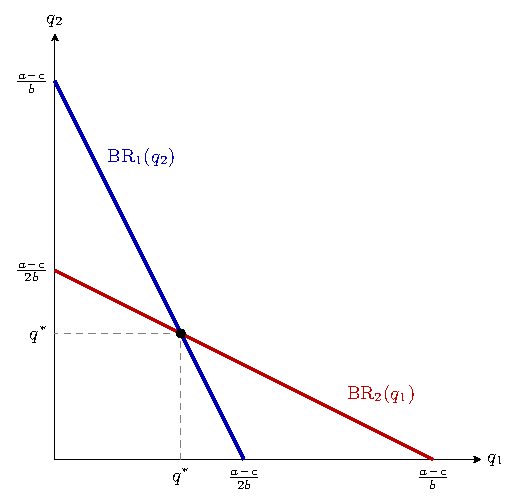
\includegraphics[width=0.6\textwidth]{figures/reaction.pdf}
  \caption{Best responses in the duopoly. The equilibrium is their intersection.}
  \label{fig:br}
\end{figure}

%=======================================================
\section{What to try in the editor}
%=======================================================

\begin{itemize}
  \item Click inside any formula, for example $\pi^{*} = (a-c)^{2}/\bigl((n+1)^{2} b\bigr)$, to see its source and a live preview while you type.
  \item Put the cursor in equation~\eqref{eq:br} and change $2b$ to $3b$: the display re-renders on each keystroke.
  \item \textbf{Cmd-click} a reference such as Proposition~\ref{prop:eq} to jump to it, or type \verb|\ref{| to get the list of labels.
  \item Add a numbered equation above \eqref{eq:demand} --- every number and reference below it updates at once, without compiling.
\end{itemize}

\begin{thebibliography}{9}
\bibitem[Cournot(1838)]{cournot1838}
Cournot, A.~A. (1838). \emph{Recherches sur les principes math\'ematiques de la th\'eorie des richesses}. Paris: Hachette.

\bibitem[Tirole(1988)]{tirole1988}
Tirole, J. (1988). \emph{The Theory of Industrial Organization}. Cambridge, MA: MIT Press.
\end{thebibliography}

\end{document}
